% Part 1, closing chapters (1 of 2): the virial partition at every scale. The thermodynamic identity is Chapter ch:virial_identity
% (p1_04_virial_identity.tex); the cosmological coupling opens Part 2 (p2_02_virial.tex, p2_02b_virial_tests.tex).
% Carried line by line from: The Virial Partition from Atoms to the Horizon (Oct 2026; sections 1-4, 6, 7 and its table);
% The Virial Partition Across Wide Range of Physical Scales (25 Feb 2026; sections 1, 2, 2.1, 2.2, Table 1, Fig. 1);
% Dark Matter and Dark Energy as Virial Partners (Mar 2026; section 2); The Thermodynamic Identity Governing the Virial Theorem
% (PRL version, 18 Mar 2026; Table I); Gravitational Decoherence and the Virial Partition (Mar 2026; sections 2.1-2.2).
% Corrections applied: errata V3, V17, V19, V29, V1, V18, V31 (docs/verification/PAPER_ERRATA.md); VIRIAL_CHECK.md items 1, 27; NBODY_TRACE.md.
% Numbers: docs/verification/scripts/verify_virial_papers.py (+ _output.txt) and verify_virial_atoms_to_horizon.py.
% Full item-by-item table: docs/book/MANIFEST_virial.md.

\chapter{One half at every scale: the virial partition}\label{ch:virial_law}

\section*{Overview}
For any system bound by a potential that falls as $1/r$, the virial theorem fixes the time-averaged kinetic energy at exactly half the magnitude of the
potential energy. This chapter follows this one half through every scale at which it can be checked: the hydrogen atom, atoms and molecules at the
Hartree--Fock limit, the Sun, white dwarfs, clusters of galaxies, the horizon of a black hole, and the horizon of the universe. The next chapter states
the thermodynamic content of the kinetic half: when a $1/r$ system binds from rest, the energy it releases equals its kinetic half, and Landauer's principle
makes that the minimum cost of the irreversible binding (Chapter~\ref{ch:virial_identity}). For a Schwarzschild black hole the Bekenstein--Hawking entropy
counted in bits, priced at $k_BT_H\ln2$ each, equals exactly $\tfrac12Mc^2$ (the Smarr relation). At the cosmic horizon the same half fixes the coupling
$\beta_m=\Omega_m/2$ of IAM, which every IAM Planck chain carries at its predicted value and which is consistent with Planck
(Part~\ref{part:2}, Chapter~\ref{ch:virial}).

IAM's Law says that every irreversible transition from a quantum superposition to a classical record pays $k_BT\ln2$ per bit, written to the nearest
encoding surface (Chapter~\ref{ch:iams_law}). The virial theorem of Clausius (1870)~\cite{Clausius1870}, the most widely tested equilibrium result in
physics, is one instance of that law. It operates in every domain where $1/r$ binding is found, and the chapters that follow show where the cost sits in it.
The 1/2 at the heart of the cosmological coupling is not a free choice. It is a mathematical theorem that holds for all $1/r$ potentials --- Coulomb and
gravitational alike --- from atomic scales ($10^{-11}$\,m) to the cosmic horizon ($10^{26}$\,m).

\section{The theorem}\label{sec:vl_theorem}
For a bound system with potential energy homogeneous of degree $k$ in the coordinates, the time average of $d(\sum_i\mathbf r_i\cdot\mathbf p_i)/dt$
vanishes, and Euler's theorem for homogeneous functions~\cite{Goldstein} gives
\begin{equation}
2\langle K\rangle=k\,\langle V\rangle .\label{eq:vl_euler}
\end{equation}
Gravity and the Coulomb interaction have $k=-1$:
\begin{equation}
2\langle K\rangle+\langle V\rangle=0,\qquad \langle K\rangle=\tfrac12|\langle V\rangle|,\qquad E=\langle K\rangle+\langle V\rangle=-\langle K\rangle .\label{eq:vl_virial}
\end{equation}
\derived\ The degree is fixed by geometry: in three spatial dimensions Gauss's law makes the field of a point source fall as $1/r^2$, so the potential falls as
$1/r$. The half does not depend on the number of bodies, their masses or the scale.

Written for an attractive potential $V\propto-r^{-n}$, which is homogeneous of degree $-n$, Eq.~\eqref{eq:vl_euler} reads
\begin{equation}
\langle T\rangle=\frac n2\,\langle|V|\rangle .\label{eq:vl_n}
\end{equation}
For the gravitational potential $V\propto-1/r$ ($n=1$), $\langle T\rangle=\tfrac12\langle|V|\rangle$. The electron--nucleus Coulomb potential is also
attractive, $V\propto-1/r$ ($n=1$), and also gives $\langle T\rangle=\tfrac12\langle|V|\rangle$. Both are $1/r$ potentials; both give exactly $1/2$. This follows
from both forces propagating in three spatial dimensions, with Gauss's law requiring a $1/r^2$ force (that is, a $1/r$ potential) from a point source. There
is no free parameter here. \derived{}

\paragraph{Homogeneity of the $1/r$ potential.} The virial coefficient of $1/2$ does not depend specifically on gravity but on the homogeneity degree of the
underlying potential. For any interaction of the form $V(r)\propto r^{-1}$ (including both Newtonian gravity and Coulomb forces), the virial theorem yields
$2K=-U$ in equilibrium. The cross-scale comparison of this chapter therefore tests the scale-independence of this homogeneity property rather than
asserting that disparate systems share identical physical mechanisms. The central question is whether empirical systems exhibit any systematic deviation
from the expected $1/2$ partition across scales. \derived

This is not a coincidence of specific systems. It follows from Euler's homogeneous function theorem applied to any potential homogeneous of degree $-1$,
and it holds exactly for any system in virial equilibrium regardless of the number of bodies, the mass distribution, or the scale. The $1/2$ is a
mathematical theorem, not an empirical fit. \derived

The half is a result for $1/r$ binding. A potential homogeneous of degree $k$ gives $2\langle K\rangle=k\langle V\rangle$, and the linear potential that
confines quarks ($k=+1$)~\cite{Eichten1978} gives the opposite partition. A quadratic potential ($k=2$) gives $\langle K\rangle=\langle V\rangle$; the
equipartition value $k_BT/2$ per quadratic degree of freedom belongs to that case, not to the $1/r$ half. The half holds for gravity and electromagnetism.
Because every atom, molecule and bond is held by electromagnetism, it holds inside every star, cell and transistor. \derived\ The same $1/2$ appears in the Bohr atom,
in a star, and in a cluster of galaxies: one mathematical structure, the $1/r$ potential, governs atoms, stars, galaxies and the cosmological coupling
constant. \prediction

\section{Atoms and molecules}\label{sec:vl_atoms}
\paragraph{Hydrogen.} The ground state has $E_1=-13.6057$\,eV, $\langle K\rangle=13.6057$\,eV and $\langle V\rangle=-27.2114$\,eV:
$\langle K\rangle/|\langle V\rangle|=1/2$. An electron captured from rest into this state emits a photon of $13.6057$\,eV, equal to its kinetic half. \calc

\paragraph{Many-electron atoms and molecules.} For the 20 atoms H--Xe and 10 molecules (H$_2$ to CO$_2$) at the Hartree--Fock limit (Clementi \& Roetti
1974~\cite{ClementiRoetti1974}; Bunge et al.\ 1993~\cite{Bunge1993}), $T/|V|=1/2$ to the precision of the tabulated energies. Equivalently, the virial ratio
\begin{equation}
\eta=-T/E=1.0000000000\qquad(\text{SD}=0\ \text{across the 20 elements and 10 molecules}).
\end{equation}
Selected values: H, $-0.500000/0.500000=1.000000$; Ne, $-128.547/128.547=1.000000$; Xe, $-7232.138/7232.138=1.000000$ (energies in hartree). Every element
agrees at machine precision, and the same calculation for the 10 molecules at equilibrium geometry gives identical results. \calc

For a converged variational wavefunction this is exact: optimizing under a uniform scaling of the coordinates enforces the quantum virial theorem. For
converged Hartree--Fock the ratio $-T/E$ must equal unity exactly, and the $1/2$ partition of the total energy between kinetic and potential halves is an
analytical consequence of the $1/r$ potential~\cite{Clausius1870}, Eq.~\eqref{eq:vl_virial}. These systems show that quantum mechanics obeys Eq.~\eqref{eq:vl_virial} with the
electrostatic interaction; they are a statement of the theorem's reach, not an independent measurement of it.

\section{Stars}\label{sec:vl_stars}
\paragraph{The Sun.} For a star in hydrostatic equilibrium the theorem gives $2K_{\rm th}+U=0$. A contracting star radiates half the gravitational energy it
releases and stores the other half as heat. For a polytrope of index 3, $U=-\tfrac32GM^2/R=-5.69\times10^{41}$\,J for the Sun; contraction alone could power
the present luminosity for $|U|/2L=24$\,Myr (23.6\,Myr; a uniform sphere, $U=-\tfrac35GM^2/R$, gives 9.4\,Myr). \calc\ The Sun is 4.6\,Gyr old
(4,568\,Myr~\cite{Bouvier2010}), so it must burn hydrogen --- the argument of Kelvin and Helmholtz, settled by the virial theorem~\cite{Kippenhahn2012}.

\paragraph{White dwarfs.} In a white dwarf the degenerate electrons become relativistic as the mass grows; the kinetic energy then scales as $1/R$ like the
gravitational energy, and Eq.~\eqref{eq:vl_virial} has a solution only at one mass,
\begin{equation}
M_{\rm Ch}=\frac{\omega_3^0\sqrt{3\pi}}{2}\left(\frac{\hbar c}{G}\right)^{3/2}\frac{1}{(\mu_em_u)^2}=1.456\,M_\odot\qquad(\mu_e=2),\label{eq:vl_chandra}
\end{equation}
with $\omega_3^0=2.01824$ (Chandrasekhar 1931~\cite{Chandrasekhar1931}, 1939~\cite{Chandrasekhar1939}). \derived\ No white dwarf has been found above it; the
most massive in the SDSS DR4 sample reach $1.33\,M_\odot$~\cite{Kepler2007}, and one of the most massive known, ZTF~J1901+1458, has $1.327$--$1.365\,M_\odot$~\cite{Caiazzo2021} \observed, and type Ia supernovae mark carbon--oxygen white dwarfs that reach it.

\section{Clusters of galaxies and simulated halos}\label{sec:vl_clusters}
Zwicky (1933)~\cite{Zwicky1933} applied Eq.~\eqref{eq:vl_virial} to the velocities of the galaxies in the Coma cluster and found far more mass than the
light suggests. Virial (dynamical) masses of clusters are now compared with weak-lensing and X-ray masses in large samples; they agree at the
tens-of-percent level, set by projection, departures from equilibrium in merging systems and non-thermal support. \observed

\paragraph{Simulated dark-matter halos.} Cosmological N-body simulations measure the virial ratio of every halo directly. Within the virial radius the
published values are $2T/|U|\approx1.1$--$1.3$, rising slowly with mass (Bett et al.\ 2007~\cite{Bett2007}; Neto et al.\ 2007~\cite{Neto2007}, ``median
slightly greater than unity''; Power, Knebe \& Knollmann 2012~\cite{Power2012}, $\eta=2T/|W|\approx1.15$ at $10^{12}$ to $1.25$ at
$10^{15}\,h^{-1}M_\odot$; Klypin et al.\ 2016~\cite{Klypin2016}). The excess over 1 is the pressure of matter still falling through the boundary: with the
surface-pressure term included, Klypin et al.\ find $2K/|W|\approx1.02$--$1.17$. Halos are called relaxed when $2T/|U|<1.35$ (Neto et al.\ 2007). \observed\
Collisionless halos, assembled without radiating, sit at the virial equilibrium to within the infall still under way.

\section{The black-hole horizon}\label{sec:vl_bh}
A Schwarzschild black hole of mass $M$ has Bekenstein--Hawking entropy and Hawking temperature~\cite{Bekenstein1973,Hawking1975}
\begin{equation}
S=\frac{k_Bc^3A}{4G\hbar}=\frac{4\pi Gk_BM^2}{\hbar c},\qquad T_H=\frac{\hbar c^3}{8\pi Gk_BM}.\label{eq:vl_bh}
\end{equation}
Counting the entropy in bits, $N=S/(k_B\ln2)$, and pricing each bit at Landauer's $k_BT_H\ln2$,
\begin{equation}
N\,k_BT_H\ln2=T_HS=\tfrac12Mc^2 .\label{eq:vl_smarr}
\end{equation}
\derived\ For one solar mass, $N=1.51\times10^{77}$ bits at $T_H=6.17\times10^{-8}$\,K; for the black holes in the Galactic center ($4.3\times10^6\,M_\odot$)
and in M87 ($6.5\times10^9\,M_\odot$) the ratio is the same, 0.5000000000. \calc\ This is the Smarr relation $Mc^2=2T_HS$ of general relativity (Smarr
1973~\cite{Smarr1973}; Bardeen, Carter \& Hawking 1973~\cite{BardeenCarterHawking1973}). Read with Landauer's principle, half of a black hole's rest energy
is the cost of the information on its horizon --- the same half as in Eq.~\eqref{eq:vl_virial}. \interp\ For a rotating (Kerr) black hole,
$Mc^2=2T_HS+2\Omega_HJ$, and the horizon share is $T_HS/Mc^2=\sqrt{1-\chi^2}/2$: 0.433 at $\chi=0.5$, 0.218 at $\chi=0.9$, 0.032 at $\chi=0.998$; the rest is
rotational energy. \calc\ The horizon thermodynamics is developed in Chapter~\ref{ch:blackholes}.

\section{The cosmic horizon}\label{sec:vl_cosmic}
IAM adds to the horizon first law of Jacobson~\cite{Jacobson1995} and of Cai \& Kim (2005)~\cite{CaiKim2005} the
entropy of the classical records produced as matter decoheres gravitationally, $-dE=T_H\,d(S_{\rm geo}+S_{\rm info})$. The share of the matter density that
enters the record term is the kinetic half of the binding energy of collapsed structure:
\begin{equation}
\beta_m=\frac{\Omega_m}{2}=0.15765\qquad(\Omega_m=0.3153,\ \text{Planck 2018}).\label{eq:vl_beta}
\end{equation}
\prediction\ The coupling is a prediction. Every IAM Planck chain carries it at this value; only the four free-$\mu_0$ test chains sample the amplitude. In the modified-CAMB (Level~2) chains on
Planck alone, the minimum $\chi^2$ of IAM (run A) is higher than that of $\Lambda$CDM (run C) by $0.54$ with the same number of parameters --- consistent with Planck --- $\sigma_8$
moves from 0.809 to 0.800, and the standard parameters are unchanged within their errors. \measured\ Its decisive test is the growth of structure measured
by Euclid: the coupling gives $\mu(z{=}0)=0.864$ ($\mu_0=-0.136$) with $\Sigma=1$. The derivation of the coupling, its predictions and its tests are
Chapters~\ref{ch:virial} and~\ref{ch:virial_tests}.

\section{The same one half across physical scales}\label{sec:vl_table}

\begin{figure}[htbp]\centering
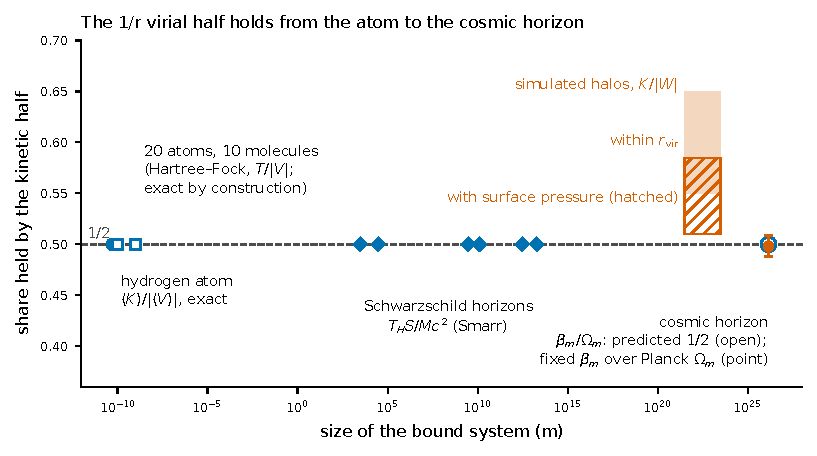
\includegraphics[width=\textwidth]{figures/part1/fig_virial_domains.pdf}
\caption{The share fixed at one half by the $1/r$ virial theorem, by size of the bound system (Table~\ref{tab:virial_domains}). Hydrogen: $\langle K\rangle/|\langle V\rangle|=13.606/27.211$ \derived. Atoms and molecules at the Hartree--Fock limit: $T/|V|=1/2$ by construction (open squares). Simulated halos: published $2K/|W|=1.1$--$1.3$ within the virial radius (shaded) and $1.02$--$1.17$ with the surface-pressure term (hatched), drawn as $K/|W|$ \observed. Schwarzschild horizons from 1 to $6.5\times10^9\,M_\odot$: $T_HS/Mc^2=0.5000000000$ (Smarr) \calc. Cosmic horizon: $\beta_m/\Omega_m=1/2$ is the prediction (open circle) \prediction; the point is the fixed $\beta_m=0.15765$ over the Level~2 Planck posterior $\Omega_m=0.3166\pm0.0065$, $0.498\pm0.010$ (\texttt{mgcamb\_validation/\allowbreak{}CHAIN\_EXTRACTION\_FINAL.csv}). White dwarfs, the Sun and galaxy clusters test the theorem through other quantities and are not drawn.}\label{fig:virial_domains}
\end{figure}
Table~\ref{tab:virial_domains} and Figure~\ref{fig:virial_domains} summarize the virial $1/2$ ratio verified across the physical systems in which $1/r$
binding has been tested, from the hydrogen atom to the cosmic horizon.

\begin{table}[htbp]\centering\small
\caption{The virial ratio for $1/r$ binding, from atoms to the cosmic horizon. Atoms and horizons \derived\ (with the Hartree--Fock values \calc), stars,
clusters and simulated halos \observed, the cosmic horizon \prediction. The electron row is the identity of Chapter~\ref{ch:virial_identity} applied at the
Compton scale \conjecture.}\label{tab:virial_domains}
\begin{tabularx}{\linewidth}{>{\raggedright\arraybackslash}X>{\raggedright\arraybackslash}p{1.6cm}>{\raggedright\arraybackslash}X>{\raggedright\arraybackslash}X}
\hline
System & Scale & Quantity & Result\\\hline
Electron (Compton scale) & $\lambda_C$ & rest energy against the Landauer cost of its decoherence loop at the horizon temperature & within $0.3\,\%$, set by $H_0$ (Chapter~\ref{ch:electronmass})\\
Hydrogen atom & $10^{-11}$--$10^{-10}$ m & $\langle K\rangle/|\langle V\rangle|$ & $1/2$ exactly (13.6057 of 27.2114\,eV)\\
20 atoms, H--Xe (Hartree--Fock limit) & $10^{-10}$ m & $T/|V|$; $-T/E$ & $1/2$; 1.0000000000 (exact for converged wavefunctions)\\
10 molecules, H$_2$--CO$_2$ & $10^{-9}$ m & $T/|V|$ & $1/2$ at equilibrium geometry\\
White dwarfs & $10^{7}$ m & Chandrasekhar mass~\cite{Chandrasekhar1931} & $1.456\,M_\odot$ ($\mu_e=2$); the most massive measured reach $1.33$--$1.37\,M_\odot$~\cite{Kepler2007,Caiazzo2021}\\
The Sun & $10^{9}$ m & $|U|/2L$~\cite{Kippenhahn2012} & 24 Myr: contraction cannot power it, so it burns hydrogen\\
Galaxy clusters (Coma; large lensing and X-ray samples) & $10^{23}$ m & dynamical against lensing and X-ray mass & agree to tens of percent (projection, mergers, non-thermal support; Zwicky 1933~\cite{Zwicky1933})\\
Simulated halos, $10^{10}$--$10^{15}M_\odot$ & $10^{21}$--$10^{23}$ m & $2K/|W|$ & $1.1$--$1.3$~\cite{Bett2007,Neto2007,Power2012}; $1.02$--$1.17$ with surface pressure~\cite{Klypin2016}\\
Schwarzschild black hole & $r_s$ & $T_HS/Mc^2$ & $1/2$ (Smarr relation~\cite{Smarr1973}; Chapter~\ref{ch:blackholes})\\
Cosmic horizon & $10^{26}$ m & $\beta_m/\Omega_m$ & $1/2$ by prediction; fixed in every IAM chain; Planck consistent, $\Delta\chi^2=+0.54$ (Chapter~\ref{ch:virial})\\\hline
\end{tabularx}
\end{table}

For converged Hartree--Fock wavefunctions the ratio is exact by construction: any wavefunction optimized under a uniform scaling of the coordinates satisfies
the quantum virial theorem. The atomic rows therefore show that quantum mechanics obeys the theorem; they are a statement of the theorem's reach, not an
independent measurement. The gravitational rows are measurements, at the precision the systems allow: the Sun to the precision of its structure model, the
clusters to tens of percent (projection, mergers, non-thermal support), the simulated halos to within the infall still under way. The span from the atom to the cluster is 33
orders of magnitude in size; carried to the horizon of the universe it runs from $10^{-11}$\,m to $10^{26}$\,m, thirty-seven decades (36.4 from the Bohr
radius to $c/H_0$). \calc\ The same mathematical theorem that governs the kinetic energy of electrons in hydrogen atoms governs the cosmological coupling
constant $\beta_m$. This universality is the key point: the fraction of energy going into the kinetic half is $1/2$ at every scale not because of a special
property of any particular system, but because every $1/r$ potential obeys the same theorem. The next chapter asks what that half is.

The virial half is the easiest place in the book to start: it is textbook mechanics, and every bound system a reader already works with carries it.
